\documentclass{article}
\usepackage[spanish]{babel}
\usepackage[utf8]{inputenc}
\usepackage[T1]{fontenc}
\usepackage{vmargin}
\usepackage{setspace}
\usepackage{enumerate}
\usepackage{graphicx}
\graphicspath{ {images/} }
\usepackage{float} 

\begin{document}
\begin{center}
\includegraphics[scale=0.3]{unison1.jpg}
\\
\vspace{0.5cm}
UNIVERSIDAD DE SONORA \\
\vspace{0.5cm}
DIVISIÓN DE CIENCIAS EXACTAS Y NATURALES \\
\vspace{0.5cm}
DEPARTAMENTO DE FÍSICA\\
\vspace{0.5cm}
LICENCIATURA EN FÍSICA\\
\vspace{0.5cm}
FÍSICA COMPUTACIONAL I
\vspace{2 cm}
\hrule
\vspace{1 cm}

{\huge \bfseries {Reporte de actividad 4}}
\\
\vspace{1 cm}
\hrule
\vspace{2 cm}
Ricardo Ruiz Hernández\\ 
\vspace{1 cm}
Profesor del curso\\
Dr. Carlos Lizárraga Celaya\\
\vspace{2 cm}
28 de febrero del 2018
\end{center}

\pagebreak
\begin{doublespace}


\hrule
\section{Introducción}

En esta práctica de laboratorio se trabajó con Shell, el cual es un intérprete de comandos. Trabajamos con scripts, para lograr familiarizarnos, puesto que más adelante, serán de suma importancia en el desarrollo de esta materia. Además, se revisó un artículo de Steve Parker, llamado: "Shell Script Tutorial". \\


\hrule
\begin{itemize}

\section{Actividad}

\item Primeramente descargamos un script, proporcionado por el profesor, llamado \textit{script1.sh}, este descargó de forma automática los datos de los 12 archivos mensuales del año 2017.
\item Seleccionamos una estación del sitio de la Universidad de Wyoming.
\item En el script sustituimos la variable STATION por la de nuestra estación seleccionada.
\item Ahora bien, el primer comando utilizado fue \textit{ls -alg}, el cual tiene la funcionalidad de mostrar los permisos del archivo en cuestión.
\\
\begin{center}
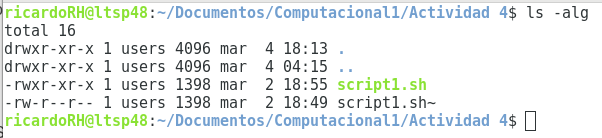
\includegraphics[scale=0.5]{act41.png}
\end{center}

\item Se puede observar que este no es un archivo ejecutable. Para cambiar esto, ejecutamos el comando chmod, para así, obtener permisos sobre el archivo de ejecución.
\\
\begin{center}
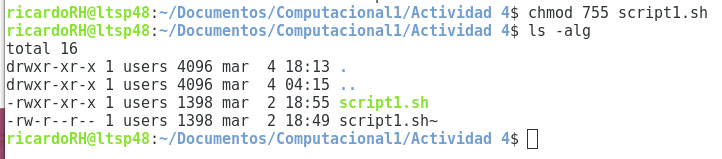
\includegraphics[scale=0.5]{act42.png}
\end{center}

\item Una vez con el permiso, ejecutamos el script, esto descargó un archivo por mes.
\\
\begin{center}
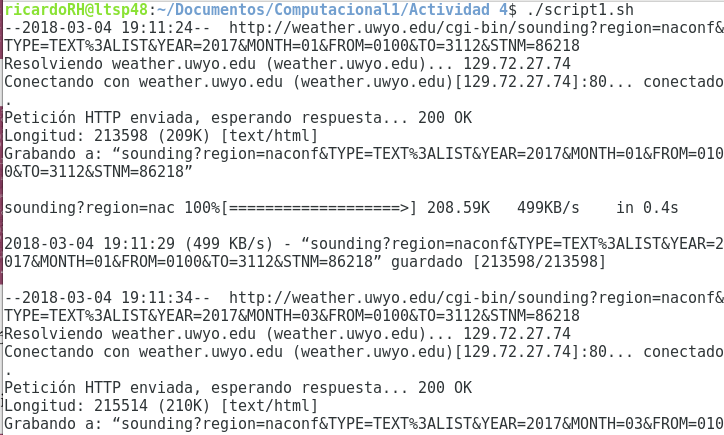
\includegraphics[scale=0.4]{act43.png}
\\
Aquí se muestran los archivos en la carpeta:
\\
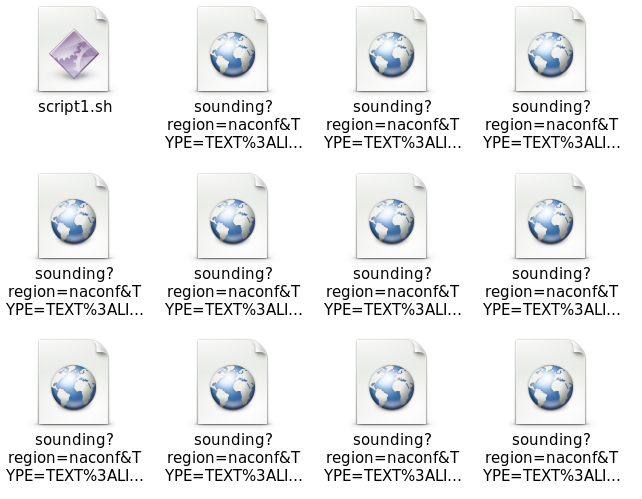
\includegraphics[scale=0.4]{act44.png}
\end{center}

\item EL siguiente comando que se utilizó fue \textit{less}, este código nos permite observar un archivo con mucho detalle y detenimiento.
\\
\begin{center}
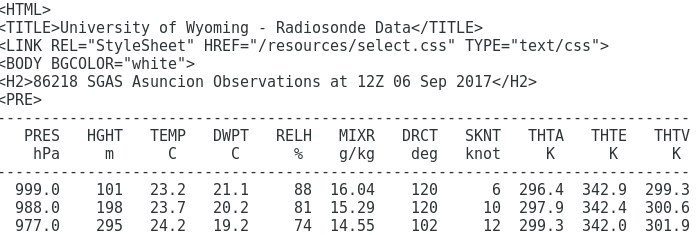
\includegraphics[scale=0.5]{act45.png}
\end{center}

\item El comando \textit{cat}, también permite observar un archivo pero de manera más rápida. Tanto en el caso anterior como en este se utilizaron los datos correspondientes al mes de septiembre.

\pagebreak
\item El comando \textit{grep} nos sirve para extraer información de un archivo. 
\\
\begin{center}
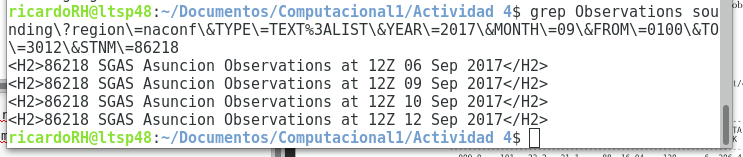
\includegraphics[scale=0.5]{act46.png}
\end{center}

\item Se utilizó el comando \textit{file}, mismo que nos brindó la información de que tipo de archivo eran los descargados.
\begin{center}
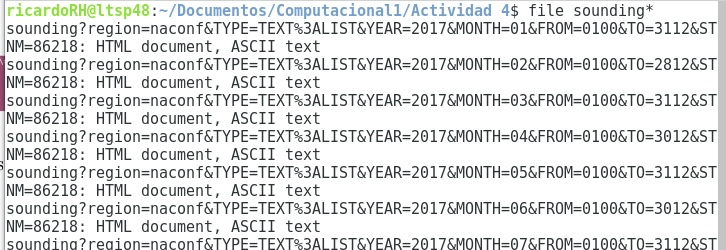
\includegraphics[scale=0.5]{act47.png}
\end{center}

\begin{center}
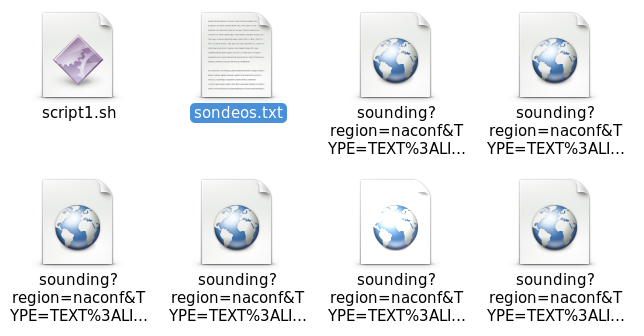
\includegraphics[scale=0.5]{act48.png}
\end{center}
\item El siguiente paso fue filtrar los renglones que nos interesa consultar del archivo de sondeos.txt, con el comando grep.
\item Modificamos el siguiente comando con nuestro número de estación (un solo renglón): 
\textit{egrep -v 'PRES|hPa' sondeos.txt | egrep'86218|Showalter|LIFT|SWEAT|K|Totals|CAPE|CINS|LFCT|CAPV|Temp|Pres|thick|Precip' > df2017.csv} 
\\
Este comando retiró los renglones que comenzaban con PRES|hPa del archivo que unió todos los demás.

\item Utilizaremos el comando \textit{cat} de nueva cuenta, para concatenar la colección de 12 archivos y almacenarlos en un solo archivo al que se le llamó \textit{sondeos.txt}. Para ellos podemos utilizar el comando: \textit{cat sounding*>sondeos.txt} 
\item Se pide hacer un script filtro.sh que automatice las acciones realizadas anteriormente, para después mediante el comando \textit{diff} comparar. Se verificó que son iguales.
\\
\begin{center}
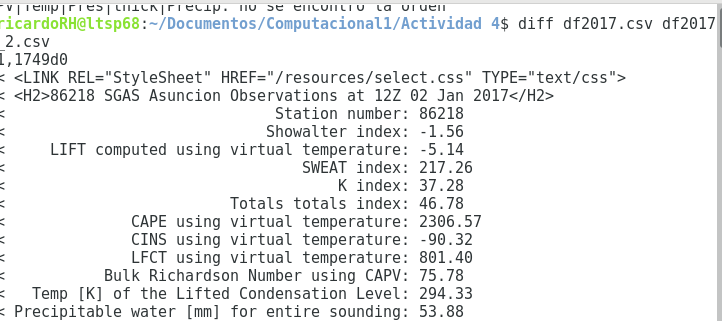
\includegraphics[scale=0.5]{act49.png}
\end{center}

\section{Comandos}
\item cat: \textit{El comando cat sirve para concatenar varios archivos y desplegarlos en pantalla.}
\item chmod: \textit{Tiene la funcionalidad de cambiar los permisos de un archivo o directorio del servidor.}
\item echo: \textit{Se utiliza para la impresión de texto en pantalla o un archivo de texto.}
\item grep: \textit{Este comando sirve para buscar en uno o más archivos las líneas que contenga un objetivo, e imprime todas las líneas que encuentra.}
\item less: \textit{Sirve para ver detalladamente (sin poder editar) el contenido de un archivo.}
\item ls: \textit{Este comando sirve para ver los archivos y directorios que tenemos dentro del que estamos trabajando.}
\item wc: \textit{Sirve para contar líneas, palabras y caracteres que contiene un archivo}
\item Redirectores: |,>: \textit{El primero sirve para separar los datos, mientras que el segundo envía datos a un archivo.}

\section{Conclusión}
A manera de conclusión puedo decir apunto que esta actividad fue realmente útil, puesto que, como dije en la parte introductoria, aprender a manejar scripts es un paso fundamental en el entendimiento de la programación en general. Los nuevos comandos aprendidos, igualmente aplían nuestro horizonte, que aunque fueron complejos en principio (en el ¿cómo?), una vez dominados, pueden llegar a ser muy fructíferos. Cabe destacar Shell, que automatizó todo, lo cual lo hizo más sencillo.

\section{Bibliografía}
Parker, S. (2017). Shell Scripting Tutorial. Shellscript.sh. Recuperado el
21 Febrero 2018, de https://www.shellscript.sh/index.html

Echo (2018). Sitio web:
https://es.wikipedia.org/wiki/Echo

Shell (computing). (2018). En.wikipedia.org. Recuperado el 20 Febrero
2018, de https://en.wikipedia.org/wiki/Shell\_(computing)



\section{Apéndice}
\begin{enumerate}
\item ¿Qué fue lo que más te llamó la atención en esta actividad?
\textit{Los scripts, sin duda, ya que, además de ser algo nuevo para mi, me parece muy interesante como automatizan las cosas.}

\item ¿Qué consideras que aprendiste?
\textit{Comandos nuevos, relacionado con los scripts.}

\item ¿Cuáles fueron las cosas que más se te dificultaron?
\textit{Familiarizarme con los nuevos comandos, pues, no sabía que estaba mal en ocasiones.}

\item ¿Cómo se podría mejorar en esta actividad?
\textit{Una base donde apoyarnos para el uso de los scripts y comandos (más teoría).}

\item ¿En general, cómo te sentiste al realizar en esta actividad? 
\textit{Al principio fue estresante, pero todo salió bien.}


\end{enumerate}



\end{itemize}
\end{doublespace}
\end{document}
